% General context + motivation

Neighbourhoods have increasingly become a central concept in social research and
targets for social
policy~\citep{sampson2012great,galster2019making,stone2015urban,looker2015nation}.
To be sure, a focus on neighbourhoods extends to the formative period of the
modern social sciences~\citep{Abbott1997}. Recent interest has at least partly
been rekindled through newly available longitudinal demographic
datasets~\citep{Logan2014,nhgis}, convenient computational
tools~\citep{rey2018spatio}, and new sources of data~\citep{Poorthuis2018}.


Yet new challenges have also emerged, especially at the convergence of research
on neighbourhood effects and neighbourhood dynamics. Neighbourhood effects
research assumes knowledge about the nature and scope of "the neighbourhood"
that presumably shapes individual outcomes~\citep{Kwan2018,Shelton2019}.
Concurrently, researchers note that neighbourhoods are not necessarily fixed
containers in which other processes occur, but themselves dynamically
evolve~\citep{Delmelle2017,Reades2019,li2018new}.  The result is to open up key
assumptions about neighbourhoods for theoretical and empirical examination: how
do we appropriately define and compare neighbourhoods at a given time?; how do
we appropriately define and compare the temporal trajectories of
neighbourhoods?; and can we do both at once, "fully
interactionally"~\citep{Abbott1997}: classify neighbourhoods now based on where
they came from and where they are going? 


In principle, much of the recent research is committed to the proposition that
neighbourhoods are open and evolving entities. Ironically, its empirical
practice tends to rely on methods that require fixed geographical regions. This
requirement is not trivial to satisfy in general, as most longitudinal datasets
are based on pre-defined tabulation areas that are routinely modified by data
collection agencies, usually to follow population changes. 

The standard approach then is to \emph{geographically harmonise} the data. This
involves interpolating existing measurements into a common set of
regions~\citep{Logan2014,Hallisey2017,Allen2018}. \revision{1.18}{Recent
computational tools have somewhat simplified this
process~\citep{rey2018spatio}}, but it still involves non-trivial questions:
which geometry to use as target, how to apportion the variables, or how to
combine data from different sources. Further, these question do not necessarily
have optimal answers. Indeed, regardless of how well this process is performed,
it still introduces errors~\citep{Logan2016}, even when additional data is
provided~\citep{eicher2001dasymetric}. Essentially, harmonisation generates
\emph{artificial data points} that can potentially lead to inaccurate results,
even though they are seldom interpreted as such. Nevertheless, because there has
been no viable alternative, and the results often appear plausible, these
concerns are overlooked. The result is that the harmonisation approach is
virtually mandatory in the current literature: \emph{"(...) tract-by-tract
comparison is not possible unless data from 2000 is interpolated to 2010
boundaries (...)"}~\citep{Dmowska2017}, \emph{"(...) This limits cross-year
comparison since data are not representative of the same spatial units. (...)"}
~\citep{Allen2018}. 

\unsure{CHECK blue text below}
\revision{1.1}{In some cases, harmonisation might seem methodologically
adequate. If a study is focused on a small subregion that is fixed in time, limiting
and modifying the data to fit that specific region of interest sounds not only
reasonable, but recommended, even if it comes at the cost of producing artificial data points. However, this view is limited in that it ignores interactions beyond the fixed
borders: each different portion of the area of interest may belong to larger
homogeneous processes beyond these arbitrarily defined borders. This effect,
along with the creation of artificial points, is caused by the geometry mismatch
between the data and the region of interest. Instead of forcing one set of
borders into another, our method sidesteps this issue by changing how the data
is represented and interpreted. It therefore allows researchers to examine changes in both the composition and extent of local areas.

The main contribution of this paper is a method for longitudinal geographical
data representation and processing that works with the original data by
leveraging a network based representation. It enables direct comparison and
temporal regionalisation without the need to match arbitrarily defined borders.
Even in the case of a small, temporally fixed, region of interest, our approach
leads to a better understanding of its dynamics by exploring the related
data-driven homogeneous regions. }

To allow a proper examination of our method and its results, we built an online
interactive system using this representation. It enables users to visualise,
interpret, and explore trajectories of neighbourhood change. This interface
helps validate our method, by allowing it to be compared to existing and future
methods. Further, it is a significant contribution to the research community: it
provides a vehicle for quickly and easily grasping complex long-term changes,
experimenting with different parameters to interactively learn from data, and
making neighbourhood change research publicly transparent. The interface thus
responds to increasing concerns about reproducibility and transparency, as well
as ongoing attention to the value of visualisation in scientific research and
communication.


We start by presenting an intuitive example of our representation in
Section~\ref{sec:introduction}, then we review the relevant literature on
longitudinal studies, data representation, clustering and regionalisation, and
spatio-temporal visualisation in Section~\ref{sec:related}. Our methodology is
introduced in detail in Section~\ref{sec:method}, along with the included
interface. Illustrative scenarios for Chicago and Toronto are presented in
Section~\ref{sec:study} and the feedback of five field experts are summarised in
Section~\ref{sec:expert}. Our prototype system is available at
\censure{\url{http://uoft.me/piccard}}, including more than forty regions in the
US and Canada. The source code is publicly available at
\censure{\url{https://github.com/fabioasdias/piccard}}.\footnote{The editors are
considering, at our request, an exception to the double-blind requirement to
allow access to the system. We provided them with the URLs of the system, code,
and documentation separately.}


\section{Intuition}
\label{sec:intuition}
While utterly simple, the network model breaks from the deeply rooted
traditional tabular paradigm in a significant way. The traditional method
requires the data to be treated as a collection of fixed entities with
properties that evolve over time -- rows in a table with temporal values as
columns. By contrast, our method represents each measurement as a separate
entity and encodes the evolution of these entities over time.

To ease the cognitive transition to this paradigm, we start with an intuitive
example of how the method works, using a small portion of a fictitious urban
region illustrated on the left part of Figure~\ref{fig:intuition}. This example
includes three different times ($t_0,t_1,t_2$), with different aggregation areas
identified as letters from A to H. For $t_0$, the initial time, we have areas A
and B, with small houses and a park, respectively. The park remains stable (B,
E, and H), but the houses are partially replaced by larger buildings (C and F). 

The aggregation areas of none of these years is clearly suitable as an
interpolation target. Adopting any of them would require merging heterogeneous
regions and/or dividing homogeneous regions. For instance, by choosing the
regions of $t_1$, A would be split to match regions C and D, which appears to be
a rather reasonable approximation in this homogeneous artificial example (even
if it commits the fallacy of division). Region F would be similarly split to
match C, but F would be split and merged with G to match D, potentially leading
to statistical measurements that do not properly represent either region. 

\revision{2.6.4}{While didactic, this example is not realistic because each
building is visible in Figure~\ref{fig:intuition}, so we know each individual of
the tabulation area, which is never the case. Further, real measurements are
seldom as homogeneous and noise-free as this artificial example.  In this
example, one possible harmonisation would split region A  in two to provide
different ancestors to C ($A_C$) and D ($A_D$). Then $A_D$ would not be
considered when analysing the evolution of C, nor $A_C$ for $D$. This is
inaccurate, because $A$ was the original state for both evolutions, and we
should not assume that these processes are disconnected.} Either way, by
splitting and merging the data to fit arbitrary borders, the harmonisation
process increases the distance between the data and reality by creating
artificial data points.


\begin{figure}
    \centering 
    \subfloat{
        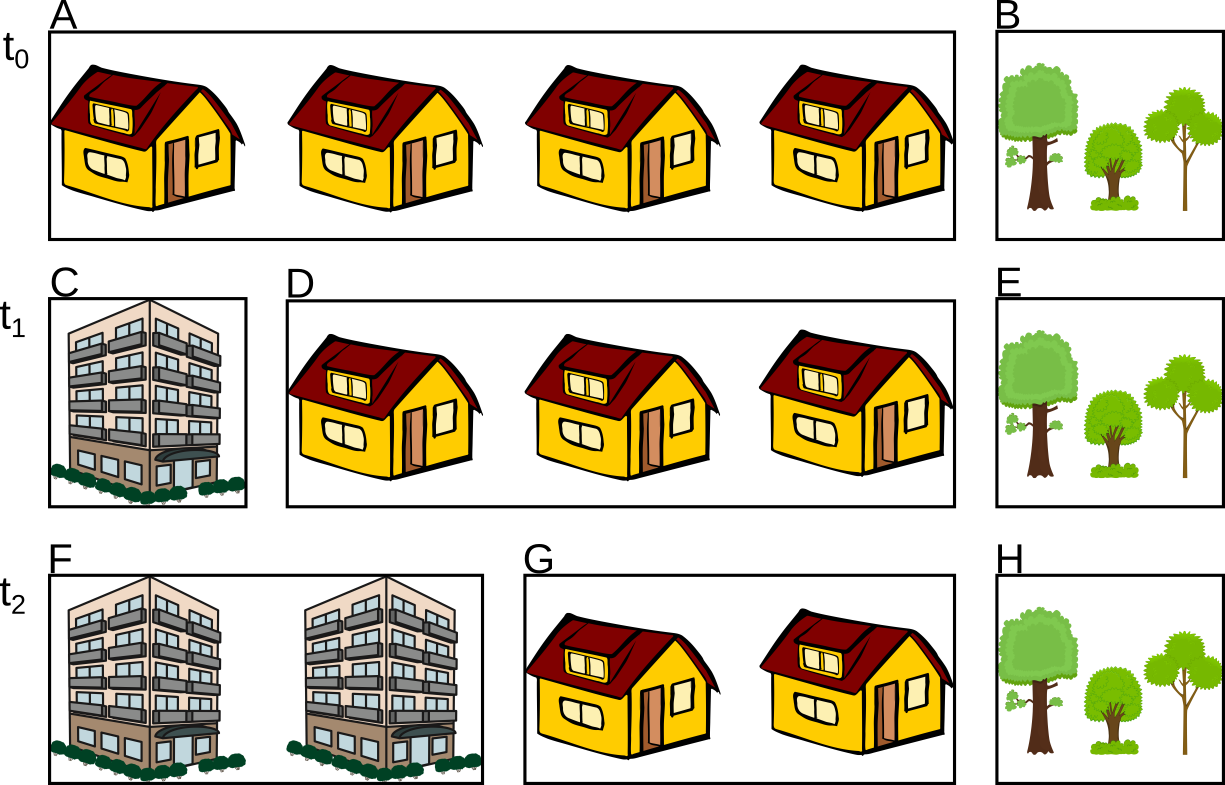
\includegraphics[width=0.475\linewidth]{intuition.png}
    }
    \subfloat{
        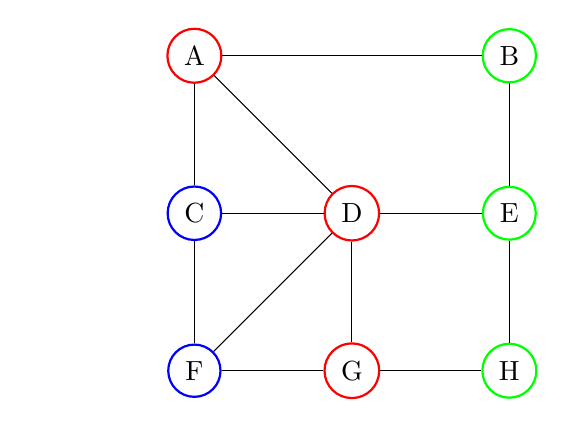
\begin{tikzpicture}
            \node (push) at (-2,0) {};
            \node [circle, draw=red, thick] (a) at (0,4) {A};
            \node [circle, draw=green, thick] (b) at (4,4) {B};
            \node [circle, draw=blue,  thick] (c) at (0,2) {C};
            \node [circle, draw=red, thick] (d) at (2,2) {D};
            \node [circle, draw=green, thick] (e) at (4,2) {E};
            \node [circle, draw=blue, thick] (f) at (0,0) {F};
            \node [circle, draw=red, thick] (g) at (2,0) {G};
            \node [circle, draw=green, thick] (h) at (4,0) {H};
            \draw (a) -- (c);
            \draw (a) -- (b);
            \draw (a) -- (d);
            \draw (b) -- (e);
            \draw (c) -- (f);
            \draw (c) -- (d);
            \draw (d) -- (f);
            \draw (d) -- (e);
            \draw (d) -- (g);
            \draw (e) -- (h);
            \draw (f) -- (g);
            \draw (g) -- (h);
        \end{tikzpicture}
    } \caption{Network based spatio-temporal data representation. \textbf{Left}:
    Three temporal stages of the evolution of a fictitious urban area, with
    aggregation areas A to H. \textbf{Right}: Network representation of the
    aggregation areas where the colours identify similar regions.
        \label{fig:intuition}}
\end{figure}

Instead, we propose a network-based representation. A \emph{network} (also
called a \emph{graph}) is a collection of entities (nodes) that are related to
each other (edges). In this case, each different aggregation area is represented
as a node and we connect nodes that have overlapping geographical areas\revision{1.2}{ in
different times or are neighbours in the same time}, leading to the network
illustrated on the right of Figure~\ref{fig:intuition}. By partitioning the
network into connected nodes that are similar, we are effectively identifying
clusters in the spatio-temporal data, as illustrated by the colours of the nodes
on the right side of Figure~\ref{fig:intuition}. Further, all the possible paths
of change can be obtained by computing sequences of nodes over time, in this
case: (A, C, F), (A, D, F), (A, D, G), and (B, E, H). This representation is
also suited for geographically consistent regions, as illustrated by the stable
park in this example, and is therefore a generalisation of the traditional
paradigm.

%I'm adding this because Jeff Allen (Farber's guy) struggled with this.
Note that the edges of this network merely encode that two regions are related.
This is binary information, there is no apportionment, no areal measurements, no
population percentages, or weights of any kind associated with the edge. Indeed,
our method also connects regions of the same time that share borders,
representing exactly that they are neighbouring areas.